
%(BEGIN_QUESTION)
% Copyright 2014, Tony R. Kuphaldt, released under the Creative Commons Attribution License (v 1.0)
% This means you may do almost anything with this work of mine, so long as you give me proper credit

En av motstandene i denne spenningsdeleren har feil og er blitt åpen krets. Basert på spenningsmålingene ved hver last, avgjør hvilken det er:

$$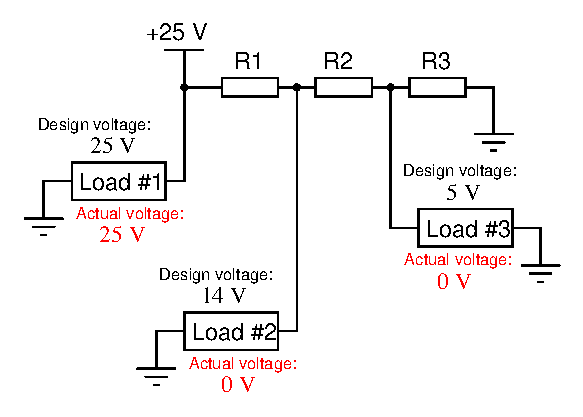
\includegraphics[width=15.5cm]{i01134x01.eps}$$

\underbar{file i01134}
%(END_QUESTION)





%(BEGIN_ANSWER)

Motstand R1 har feil og er åpen. Det ser vi fordi bare last \#1 får effekt; de to andre lastene er helt ``døde''.

%(END_ANSWER)





%(BEGIN_NOTES)

Diskuter med elevene hvordan de kunne forutsi at R1 var feilmotstanden. Finnes det noen tydelig ledetråd i diagrammet som peker på R1?

%INDEX% Elektronikkrepetisjon: serie-parallellkretser

%(END_NOTES)


